\begin{figure}
\begin{subfigure}{.5\textwidth}
  \centering
  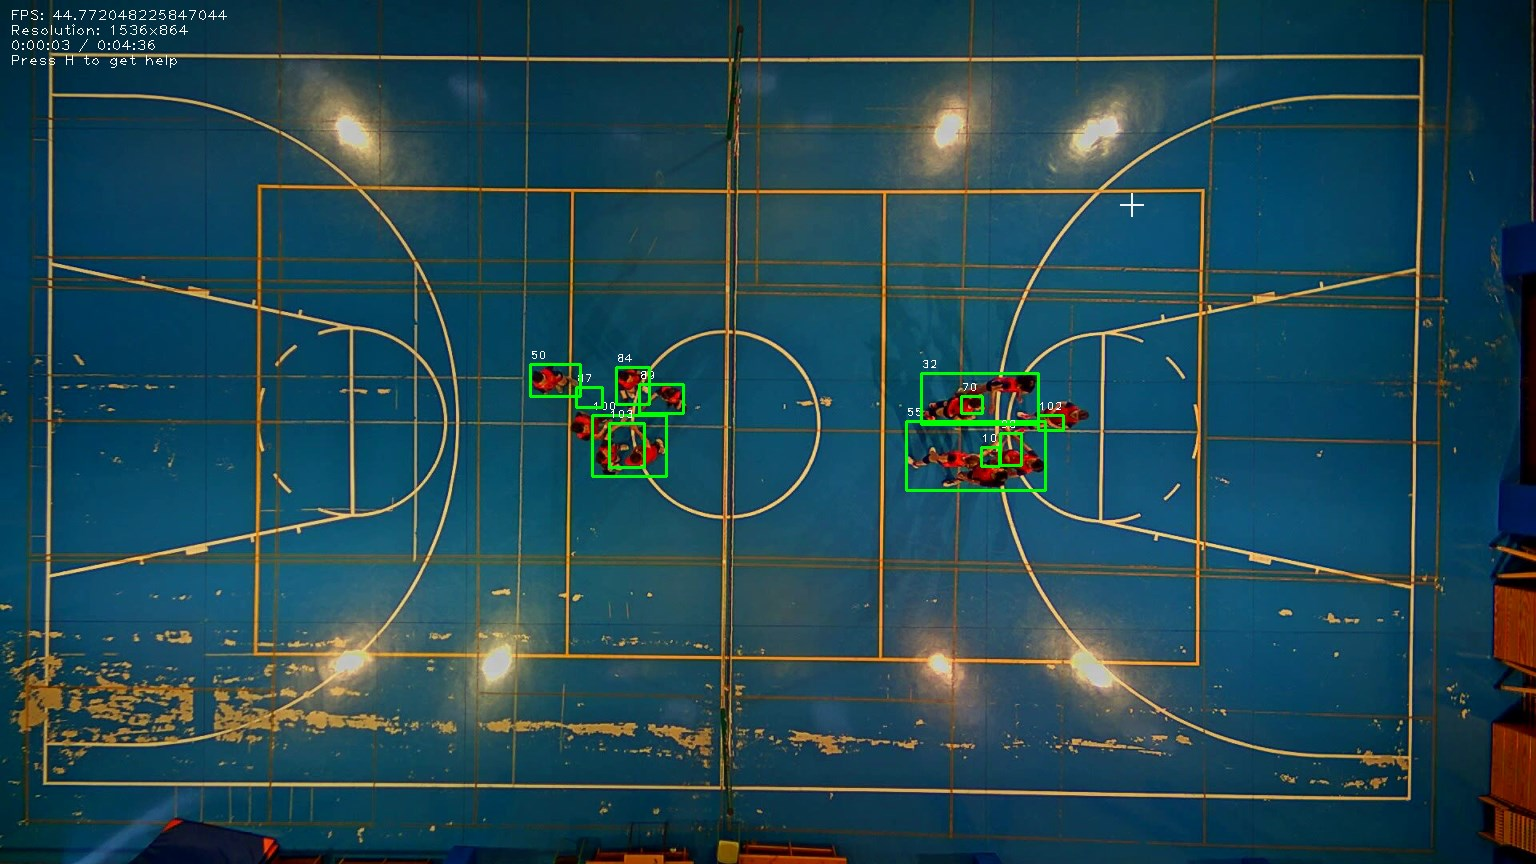
\includegraphics[width=.9\linewidth]{images/nonms}
  \caption { }
  \label{fig:nms1a}
\end{subfigure}%
\begin{subfigure}{.5\textwidth}
  \centering
  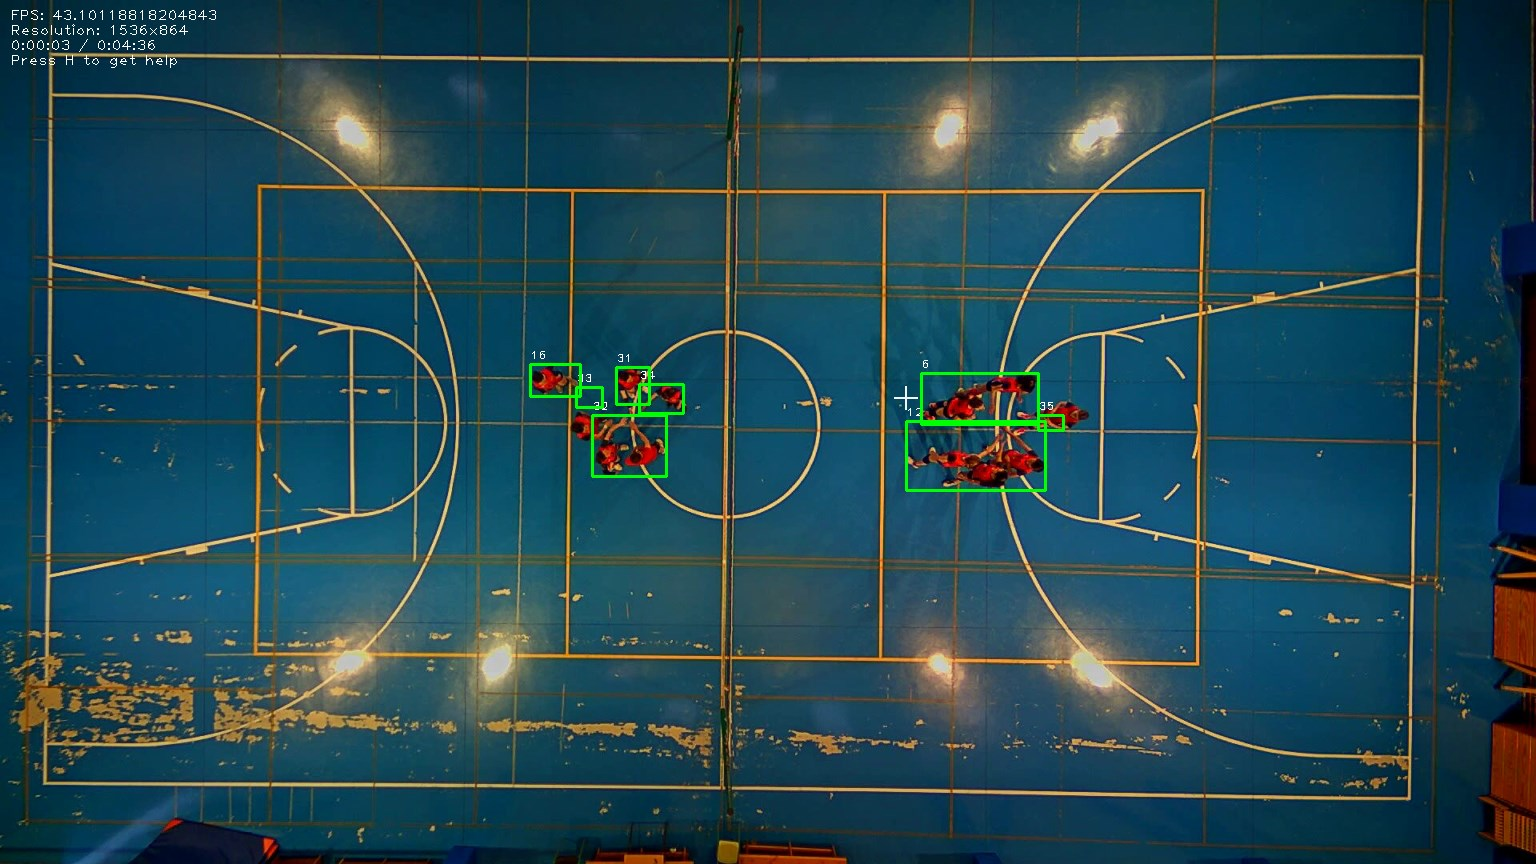
\includegraphics[width=.9\linewidth]{images/nms}
  \caption { }
  \label{fig:nms1b}
\end{subfigure}
\caption{Comparativa de la salida del vídeo antes (a) y después (b) de aplicar la operación de supresión de no máximos }
\label{fig:nms}
\end{figure}